\documentclass[aspectratio=169]{beamer}
\usepackage[utf8]{inputenc}
\usepackage{lmodern}
\usepackage[T1]{fontenc}
\usepackage{listings}
\usepackage{tikz}
\usetikzlibrary{arrows.meta, positioning, shapes.geometric, calc}

% Set path to find the theme
\makeatletter
\def\input@path{{../BeamerTemplate/theme/}}
\makeatother

\usetheme{CleanEasy}
\input{../BeamerTemplate/configs/configs}

% Listings configuration
\lstset{
    basicstyle=\ttfamily\footnotesize,
    keywordstyle=\color{blue},
    commentstyle=\color{gray},
    stringstyle=\color{red},
    showstringspaces=false,
    breaklines=true,
    frame=single,
    numbers=left,
    numberstyle=\tiny\color{gray}
}

\title{B-Trees and B+ Trees}
\subtitle{Disk-Friendly Balanced Trees for Indexing and Storage}
\author{Minseok Jeon}
\institute{DGIST}
\date{\today}

\begin{document}

\begin{frame}
  \titlepage
\end{frame}

\begin{frame}{Table of Contents}
  \tableofcontents
\end{frame}

\section{Introduction}

\begin{frame}{What are B-Trees?}
  \textbf{B-Trees}: Self-balancing tree data structures optimized for disk storage

  \vspace{0.3cm}
  \textbf{Key Characteristics:}
  \begin{itemize}
    \item Generalization of binary search trees (multi-way trees)
    \item Designed for systems with slow, block-based storage (disks)
    \item Minimize disk I/O operations
    \item All leaves at the same depth (perfectly balanced)
    \item High branching factor (many children per node)
  \end{itemize}

  \vspace{0.3cm}
  \textbf{Why B-Trees?}
  \begin{itemize}
    \item Disk access is 100,000x slower than RAM
    \item Reading a disk block has fixed cost (4KB, 8KB)
    \item Solution: Pack many keys per node to reduce tree height
  \end{itemize}
\end{frame}

\begin{frame}{Historical Context}
  \textbf{Invented in 1970 by Rudolf Bayer and Edward McCreight}

  \vspace{0.3cm}
  \textbf{Timeline:}
  \begin{itemize}
    \item \textbf{1970}: B-Tree invented at Boeing Research Labs
    \item \textbf{1979}: B+ Tree variant introduced
    \item \textbf{1980s}: Adopted by major database systems
    \item \textbf{Today}: Standard for database indexes and filesystems
  \end{itemize}

  \vspace{0.3cm}
  \textbf{Impact:}
  \begin{itemize}
    \item Revolutionized database indexing
    \item Enabled efficient large-scale data storage
    \item Foundation of modern relational databases
  \end{itemize}
\end{frame}

\section{Node Structure and Order}

\begin{frame}{Node Structure and Order}
  \textbf{Order (m)}: Maximum number of children a node can have

  \vspace{0.3cm}
  \textbf{Node Properties:}
  \begin{itemize}
    \item Each node contains up to $m-1$ keys
    \item Each node has up to $m$ children
    \item Keys stored in sorted order
    \item \textbf{Internal nodes}: keys + child pointers
    \item \textbf{Leaf nodes}: keys + data (or pointers to data)
  \end{itemize}

  \vspace{0.3cm}
  \textbf{Common Order Values:}
  \begin{itemize}
    \item Small trees: $m = 3, 5, 7$
    \item Disk-based systems: $m = 100$ to $1000$
  \end{itemize}
\end{frame}

\begin{frame}[fragile]{B-Tree Node Implementation}
\begin{lstlisting}[language=Python, basicstyle=\ttfamily\tiny]
class BTreeNode:
    def __init__(self, order, is_leaf=False):
        self.order = order              # Maximum children
        self.keys = []                  # Sorted keys
        self.children = []              # Child pointers
        self.is_leaf = is_leaf          # Leaf flag
        self.n = 0                      # Current number of keys
\end{lstlisting}

\vspace{0.3cm}
\textbf{Node Constraints:}
\begin{itemize}
  \item \textbf{Root}: 1 to $m-1$ keys, 2 to $m$ children (if not leaf)
  \item \textbf{Internal nodes}: $\lceil m/2 \rceil - 1$ to $m-1$ keys, $\lceil m/2 \rceil$ to $m$ children
  \item \textbf{Leaf nodes}: $\lceil m/2 \rceil - 1$ to $m-1$ keys
  \item \textbf{All leaves at same depth} (balanced)
\end{itemize}
\end{frame}

\begin{frame}{Example: B-Tree of Order 5}
  \textbf{Node Structure ($m=5$):}
  \begin{itemize}
    \item Min keys (internal): $\lceil 5/2 \rceil - 1 = 2$
    \item Max keys: $4$
    \item Min children (internal): $\lceil 5/2 \rceil = 3$
    \item Max children: $5$
  \end{itemize}

  \vspace{0.3cm}
  \textbf{Example Node:}
  \begin{center}
  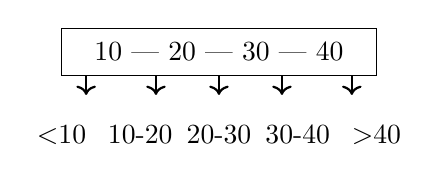
\begin{tikzpicture}[scale=0.8]
    % Node
    \node[draw, minimum width=4cm, minimum height=0.6cm] (node) at (0,0) {10 | 20 | 30 | 40};

    % Children labels
    \node[below=0.5cm of node, xshift=-2cm] {$<$10};
    \node[below=0.5cm of node, xshift=-1cm] {10-20};
    \node[below=0.5cm of node] {20-30};
    \node[below=0.5cm of node, xshift=1cm] {30-40};
    \node[below=0.5cm of node, xshift=2cm] {$>$40};

    % Arrows
    \draw[->,thick] (node.south west) ++ (0.4,0) -- ++(0,-0.3);
    \draw[->,thick] (node.south) ++ (-1,0) -- ++(0,-0.3);
    \draw[->,thick] (node.south) -- ++(0,-0.3);
    \draw[->,thick] (node.south) ++ (1,0) -- ++(0,-0.3);
    \draw[->,thick] (node.south east) ++ (-0.4,0) -- ++(0,-0.3);
  \end{tikzpicture}
  \end{center}
\end{frame}

\begin{frame}{Memory Layout Considerations}
  \textbf{Node Size Matching Disk Block Size}

  \vspace{0.3cm}
  \textbf{Example Calculation:}
  \begin{itemize}
    \item Disk block size: 4KB (4096 bytes)
    \item Key size: 8 bytes
    \item Pointer size: 8 bytes
    \item Available space: $\approx$ 4000 bytes (accounting for metadata)
  \end{itemize}

  \vspace{0.3cm}
  \textbf{Order Calculation:}
  \begin{itemize}
    \item Node contains: $m$ pointers + $(m-1)$ keys
    \item Space: $8m + 8(m-1) = 16m - 8$ bytes
    \item $16m - 8 \leq 4000$
    \item $m \leq 250.5$
    \item \textbf{Order $m \approx 250$}
  \end{itemize}

  \vspace{0.3cm}
  \textbf{Impact:} 250-way branching means very shallow trees!
\end{frame}

\section{Insertion and Split}

\begin{frame}{Insertion Algorithm Overview}
  \textbf{Steps:}
  \begin{enumerate}
    \item \textbf{Search for leaf}: Traverse tree to find appropriate leaf node
    \item \textbf{Insert in leaf}: Add key in sorted position
    \item \textbf{Check overflow}: If node has $m$ keys (too many), split
    \item \textbf{Split operation}:
    \begin{itemize}
      \item Create new node
      \item Move upper half of keys to new node
      \item Promote middle key to parent
      \item If parent overflows, split recursively up to root
    \end{itemize}
  \end{enumerate}

  \vspace{0.3cm}
  \textbf{Key Property:} Splits propagate upward, may create new root
\end{frame}

\begin{frame}[fragile]{Insertion Implementation - Main Function}
\begin{lstlisting}[language=Python, basicstyle=\ttfamily\tiny]
def insert(root, key):
    # If root is full, split it
    if root.n == root.order - 1:
        new_root = BTreeNode(root.order)
        new_root.children.append(root)
        split_child(new_root, 0)
        root = new_root

    insert_non_full(root, key)
    return root

def insert_non_full(node, key):
    if node.is_leaf:
        # Insert key in sorted position
        node.keys.insert(bisect_left(node.keys, key), key)
        node.n += 1
    else:
        # Find child to insert into
        i = bisect_left(node.keys, key)
        if node.children[i].n == node.order - 1:
            split_child(node, i)
            if key > node.keys[i]:
                i += 1
        insert_non_full(node.children[i], key)
\end{lstlisting}
\end{frame}

\begin{frame}[fragile]{Split Child Operation}
\begin{lstlisting}[language=Python, basicstyle=\ttfamily\tiny]
def split_child(parent, index):
    full_child = parent.children[index]
    new_child = BTreeNode(full_child.order, full_child.is_leaf)

    mid = full_child.order // 2

    # Promote middle key to parent
    parent.keys.insert(index, full_child.keys[mid])
    parent.children.insert(index + 1, new_child)

    # Split keys and children
    new_child.keys = full_child.keys[mid+1:]
    full_child.keys = full_child.keys[:mid]

    if not full_child.is_leaf:
        new_child.children = full_child.children[mid+1:]
        full_child.children = full_child.children[:mid+1]

    # Update counts
    new_child.n = len(new_child.keys)
    full_child.n = len(full_child.keys)
    parent.n += 1
\end{lstlisting}
\end{frame}

\begin{frame}{Insertion Example: Step-by-Step}
  \textbf{Insert into B-Tree of order 3 (max 2 keys per node)}

  \vspace{0.2cm}
  \textbf{Initial tree:}
  \begin{center}
  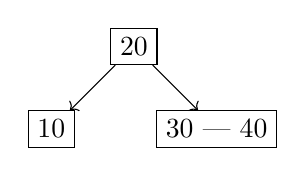
\begin{tikzpicture}[scale=0.7]
    \node[draw] (root) at (0,0) {20};
    \node[draw] (left) at (-1.5,-1.5) {10};
    \node[draw] (right) at (1.5,-1.5) {30 | 40};

    \draw[->] (root) -- (left);
    \draw[->] (root) -- (right);
  \end{tikzpicture}
  \end{center}

  \textbf{Insert 35:}
  \begin{itemize}
    \item Navigate to right child [30 | 40]
    \item Insert 35: [30 | 35 | 40] - overflow!
    \item Split: promote 35 to parent
  \end{itemize}

  \vspace{0.2cm}
  \textbf{After split:}
  \begin{center}
  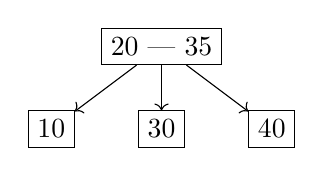
\begin{tikzpicture}[scale=0.7]
    \node[draw] (root) at (0,0) {20 | 35};
    \node[draw] (l) at (-2,-1.5) {10};
    \node[draw] (m) at (0,-1.5) {30};
    \node[draw] (r) at (2,-1.5) {40};

    \draw[->] (root) -- (l);
    \draw[->] (root) -- (m);
    \draw[->] (root) -- (r);
  \end{tikzpicture}
  \end{center}
\end{frame}

\section{Deletion and Merge}

\begin{frame}{Deletion Algorithm Overview}
  \textbf{More Complex than Insertion - Three Cases:}

  \vspace{0.3cm}
  \textbf{Case 1: Key in Leaf Node}
  \begin{itemize}
    \item Simply remove the key
    \item Check for underflow
  \end{itemize}

  \vspace{0.3cm}
  \textbf{Case 2: Key in Internal Node}
  \begin{itemize}
    \item Replace with predecessor or successor
    \item Delete predecessor/successor from leaf
    \item Handle any resulting underflow
  \end{itemize}

  \vspace{0.3cm}
  \textbf{Case 3: Underflow Handling}
  \begin{itemize}
    \item Node has fewer than $\lceil m/2 \rceil - 1$ keys
    \item \textbf{Option A}: Borrow from sibling (if sibling has extra keys)
    \item \textbf{Option B}: Merge with sibling (if sibling at minimum)
  \end{itemize}
\end{frame}

\begin{frame}{Deletion Case 1: Delete from Leaf}
  \textbf{Simple Case - No Underflow}

  \vspace{0.3cm}
  \textbf{Before:}
  \begin{center}
  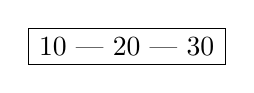
\begin{tikzpicture}[scale=0.8]
    \node[draw, minimum width=2.5cm] at (0,0) {10 | 20 | 30};
  \end{tikzpicture}
  \end{center}

  \vspace{0.2cm}
  \textbf{Delete 20}

  \vspace{0.2cm}
  \textbf{After:}
  \begin{center}
  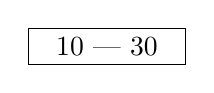
\begin{tikzpicture}[scale=0.8]
    \node[draw, minimum width=2cm] at (0,0) {10 | 30};
  \end{tikzpicture}
  \end{center}

  \vspace{0.3cm}
  \textbf{Condition:} Resulting node still has $\geq \lceil m/2 \rceil - 1$ keys
\end{frame}

\begin{frame}{Deletion Case 2: Delete from Internal Node}
  \textbf{Replace with Predecessor}

  \vspace{0.3cm}
  \textbf{Before:}
  \begin{center}
  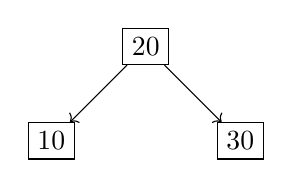
\begin{tikzpicture}[scale=0.8]
    \node[draw] (root) at (0,0) {20};
    \node[draw] (left) at (-1.5,-1.5) {10};
    \node[draw] (right) at (1.5,-1.5) {30};

    \draw[->] (root) -- (left);
    \draw[->] (root) -- (right);
  \end{tikzpicture}
  \end{center}

  \textbf{Delete 20:}
  \begin{itemize}
    \item Find predecessor (largest in left subtree): 10
    \item Replace 20 with 10
    \item Delete 10 from leaf
  \end{itemize}

  \vspace{0.2cm}
  \textbf{After:}
  \begin{center}
  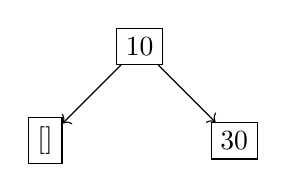
\begin{tikzpicture}[scale=0.8]
    \node[draw] (root) at (0,0) {10};
    \node[draw] (left) at (-1.5,-1.5) {[]};
    \node[draw] (right) at (1.5,-1.5) {30};

    \draw[->] (root) -- (left);
    \draw[->] (root) -- (right);
  \end{tikzpicture}
  \end{center}

  \textbf{Note:} Left child underflow requires handling
\end{frame}

\begin{frame}{Deletion Case 3: Merge Siblings}
  \textbf{When Underflow Occurs and Sibling Can't Lend}

  \vspace{0.3cm}
  \textbf{Before:}
  \begin{center}
  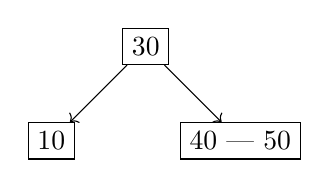
\begin{tikzpicture}[scale=0.8]
    \node[draw] (root) at (0,0) {30};
    \node[draw] (left) at (-1.5,-1.5) {10};
    \node[draw] (right) at (1.5,-1.5) {40 | 50};

    \draw[->] (root) -- (left);
    \draw[->] (root) -- (right);
  \end{tikzpicture}
  \end{center}

  \textbf{Delete 10:}
  \begin{itemize}
    \item Left child becomes empty (underflow)
    \item Right sibling has only 2 keys (can't lend)
    \item \textbf{Solution}: Merge left and right with parent key 30
  \end{itemize}

  \vspace{0.2cm}
  \textbf{After merge:}
  \begin{center}
  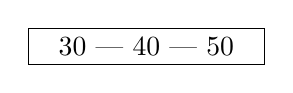
\begin{tikzpicture}[scale=0.8]
    \node[draw, minimum width=3cm] at (0,0) {30 | 40 | 50};
  \end{tikzpicture}
  \end{center}

  \textbf{Result:} Parent key pulled down, siblings merged
\end{frame}

\section{Height and Complexity}

\begin{frame}{Height Formula and Analysis}
  \textbf{For $n$ keys and order $m$:}

  \vspace{0.3cm}
  \textbf{Height Bounds:}
  \begin{itemize}
    \item \textbf{Minimum height}: $\log_m(n+1)$ (fully packed nodes)
    \item \textbf{Maximum height}: $\log_{\lceil m/2 \rceil}((n+1)/2)$ (minimum occupancy)
  \end{itemize}

  \vspace{0.3cm}
  \textbf{Example: 1 Million Keys, Order $m=100$}
  \begin{itemize}
    \item Minimum children per internal node: $\lceil 100/2 \rceil = 50$
    \item Height $\leq \log_{50}(1,000,000) \approx 3.5$
    \item \textbf{Only 4 disk accesses to find any key!}
  \end{itemize}

  \vspace{0.3cm}
  \textbf{Key Insight:}
  \begin{itemize}
    \item High branching factor dramatically reduces height
    \item Each level = one disk I/O
    \item Shallow tree = fast queries
  \end{itemize}
\end{frame}

\begin{frame}{Time Complexity Analysis}
  \begin{center}
  \begin{tabular}{|l|c|c|}
    \hline
    \textbf{Operation} & \textbf{Time Complexity} & \textbf{Disk I/Os} \\
    \hline
    Search & $O(\log_m n)$ & $O(\log_m n)$ \\
    \hline
    Insert & $O(\log_m n)$ & $O(\log_m n)$ \\
    \hline
    Delete & $O(\log_m n)$ & $O(\log_m n)$ \\
    \hline
    Range Scan & $O(\log_m n + k)$ & $O(\log_m n + k/b)$ \\
    \hline
  \end{tabular}
  \end{center}

  \vspace{0.3cm}
  \textbf{Where:}
  \begin{itemize}
    \item $n$ = number of keys
    \item $m$ = order (branching factor)
    \item $k$ = number of results in range query
    \item $b$ = keys per block
  \end{itemize}

  \vspace{0.3cm}
  \textbf{Space Complexity:} $O(n)$
  \begin{itemize}
    \item Minimum 50\% space utilization (except root)
    \item Average 67-75\% utilization in practice
  \end{itemize}
\end{frame}

\begin{frame}{Comparison with Binary Search Trees}
  \begin{center}
  \begin{tabular}{|l|c|c|}
    \hline
    \textbf{Tree Type} & \textbf{Height for 1M keys} & \textbf{Disk I/Os} \\
    \hline
    Binary tree (balanced) & $\log_2(10^6) \approx 20$ & 20 \\
    \hline
    B-Tree ($m=100$) & $\log_{100}(10^6) \approx 3$ & 3 \\
    \hline
    B-Tree ($m=1000$) & $\log_{1000}(10^6) \approx 2$ & 2 \\
    \hline
  \end{tabular}
  \end{center}

  \vspace{0.3cm}
  \textbf{Why B-Trees are Efficient:}
  \begin{itemize}
    \item \textbf{High branching factor} $\rightarrow$ shallow tree
    \item \textbf{Fewer disk accesses} (dominant cost in I/O-bound systems)
    \item \textbf{Each node fits in one disk block} (4KB, 8KB)
    \item \textbf{Sequential access within nodes} (cache-friendly)
  \end{itemize}

  \vspace{0.3cm}
  \textbf{Result:} 6-7x reduction in disk I/Os compared to balanced BST
\end{frame}

\section{B-Tree vs B+ Tree}

\begin{frame}{B-Tree Structure}
  \textbf{Classic B-Tree Characteristics:}

  \vspace{0.3cm}
  \textbf{Structure:}
  \begin{itemize}
    \item Keys and data in \textbf{all nodes} (internal + leaf)
    \item Each key appears \textbf{exactly once}
    \item No linked list between leaves
  \end{itemize}

  \vspace{0.3cm}
  \textbf{Advantages:}
  \begin{itemize}
    \item Better for \textbf{exact-match queries} (may find in internal node)
    \item Slightly less space (no duplicate keys)
  \end{itemize}

  \vspace{0.3cm}
  \textbf{Disadvantages:}
  \begin{itemize}
    \item Range queries less efficient
    \item Variable-size records complicate node management
    \item Must traverse tree for sequential access
  \end{itemize}
\end{frame}

\begin{frame}{B+ Tree Structure}
  \textbf{Enhanced Variant for Databases:}

  \vspace{0.3cm}
  \textbf{Structure:}
  \begin{itemize}
    \item All data in \textbf{leaf nodes only}
    \item Internal nodes contain only keys (for routing)
    \item Keys may be duplicated (in internal + leaf)
    \item \textbf{Leaves linked in sorted order} (doubly linked list)
  \end{itemize}

  \vspace{0.3cm}
  \textbf{Advantages:}
  \begin{itemize}
    \item \textbf{Excellent for range queries} (scan linked leaves)
    \item More keys per internal node (no data overhead)
    \item Sequential access via leaf chain
    \item Consistent performance (always reach leaf)
  \end{itemize}

  \vspace{0.3cm}
  \textbf{Disadvantages:}
  \begin{itemize}
    \item Duplicate keys use extra space
    \item Always traverse to leaf (even if key in internal node)
  \end{itemize}
\end{frame}

\begin{frame}{Visual Comparison}
  \textbf{B-Tree (order 3):}
  \begin{center}
  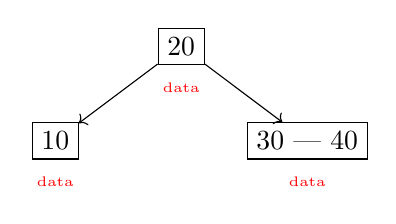
\begin{tikzpicture}[scale=0.8]
    \node[draw] (root) at (0,0) {20};
    \node[draw] (left) at (-2,-1.5) {10};
    \node[draw] (right) at (2,-1.5) {30 | 40};

    \draw[->] (root) -- (left);
    \draw[->] (root) -- (right);

    \node[below=0.1cm of root, text=red] {\tiny data};
    \node[below=0.1cm of left, text=red] {\tiny data};
    \node[below=0.1cm of right, text=red] {\tiny data};
  \end{tikzpicture}
  \end{center}
  \textbf{All nodes contain data}

  \vspace{0.5cm}
  \textbf{B+ Tree (order 3):}
  \begin{center}
  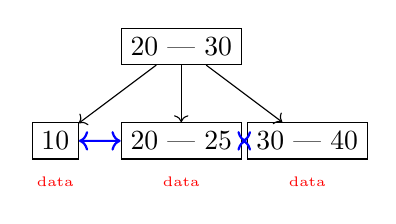
\begin{tikzpicture}[scale=0.8]
    \node[draw] (root) at (0,0) {20 | 30};
    \node[draw] (l) at (-2,-1.5) {10};
    \node[draw] (m) at (0,-1.5) {20 | 25};
    \node[draw] (r) at (2,-1.5) {30 | 40};

    \draw[->] (root) -- (l);
    \draw[->] (root) -- (m);
    \draw[->] (root) -- (r);

    \draw[<->, thick, blue] (l) -- (m);
    \draw[<->, thick, blue] (m) -- (r);

    \node[below=0.1cm of l, text=red] {\tiny data};
    \node[below=0.1cm of m, text=red] {\tiny data};
    \node[below=0.1cm of r, text=red] {\tiny data};
  \end{tikzpicture}
  \end{center}
  \textbf{Only leaves contain data, leaves are linked}
\end{frame}

\begin{frame}{Detailed Comparison Table}
  \begin{center}
  \begin{tabular}{|l|c|c|}
    \hline
    \textbf{Feature} & \textbf{B-Tree} & \textbf{B+ Tree} \\
    \hline
    Data location & All nodes & Leaf only \\
    \hline
    Internal nodes & Keys + data & Keys only \\
    \hline
    Key duplication & No & Yes \\
    \hline
    Leaf linkage & No & Yes \\
    \hline
    Keys per internal & Fewer & More \\
    \hline
    Range queries & $O(\log n + k)$ & $O(\log n + k/b)$ \\
    \hline
    Point queries & Faster & Always to leaf \\
    \hline
    Sequential access & Poor & Excellent \\
    \hline
    Use case & General & DB/Filesystem \\
    \hline
  \end{tabular}
  \end{center}
\end{frame}

\begin{frame}{Why Databases Prefer B+ Trees}
  \textbf{Five Key Reasons:}

  \vspace{0.3cm}
  \textbf{1. Range Queries:}
  \begin{itemize}
    \item Common in SQL: \texttt{SELECT * WHERE age BETWEEN 20 AND 30}
    \item Efficient leaf chain scanning
  \end{itemize}

  \textbf{2. Sequential Scans:}
  \begin{itemize}
    \item Full table scans via leaf chain
    \item No need to traverse internal nodes repeatedly
  \end{itemize}

  \textbf{3. Higher Fanout:}
  \begin{itemize}
    \item More keys per internal node $\rightarrow$ shorter tree
    \item Internal nodes don't store data
  \end{itemize}

  \textbf{4. Predictable Performance:}
  \begin{itemize}
    \item Always same depth to leaf
    \item Consistent query response times
  \end{itemize}

  \textbf{5. Easier Concurrency:}
  \begin{itemize}
    \item Lock leaves independently
    \item Better parallelism for reads
  \end{itemize}
\end{frame}

\section{Range Scans and Storage Locality}

\begin{frame}{Range Query in B+ Tree}
  \textbf{Algorithm:}
  \begin{enumerate}
    \item \textbf{Find start key}: $O(\log_m n)$ - traverse to leaf
    \item \textbf{Scan leaves}: Follow linked list until end key
    \item \textbf{Total cost}: $O(\log_m n + k)$ where $k$ = results
  \end{enumerate}

  \vspace{0.3cm}
  \textbf{Example Query:}
  \begin{center}
  \texttt{SELECT * FROM users WHERE age BETWEEN 25 AND 35}
  \end{center}

  \textbf{Execution Steps:}
  \begin{itemize}
    \item Step 1: Search for \texttt{age=25} $\rightarrow$ reach leaf $L_1$
    \item Step 2: Scan $L_1 \rightarrow L_2 \rightarrow L_3$ until \texttt{age > 35}
    \item Step 3: Return all records found
  \end{itemize}

  \vspace{0.3cm}
  \textbf{Disk I/Os:}
  \begin{itemize}
    \item 1 (root) + 1 (internal) + 1 (leaf) + $k/b$ (scan)
    \item Much better than $k$ separate point queries!
  \end{itemize}
\end{frame}

\begin{frame}{Range Query in B-Tree}
  \textbf{Less Efficient - Must Use In-Order Traversal}

  \vspace{0.3cm}
  \textbf{Problem:}
  \begin{itemize}
    \item No leaf linkage
    \item Must jump between internal and leaf nodes
    \item Random access pattern
  \end{itemize}

  \vspace{0.3cm}
  \textbf{Complexity:}
  \begin{itemize}
    \item $O(\log_m n + k \log_m n)$ - revisit internal nodes
    \item Much worse than B+ Tree for large ranges
  \end{itemize}

  \vspace{0.3cm}
  \textbf{Example:}
  \begin{itemize}
    \item Range query with 1000 results
    \item B+ Tree: $3 + 10 = 13$ I/Os (assuming 100 keys/block)
    \item B-Tree: $3 + 1000 \times 3 = 3003$ I/Os
  \end{itemize}
\end{frame}

\begin{frame}{Storage Locality Benefits}
  \textbf{Sequential Disk Access:}
  \begin{itemize}
    \item Leaves stored contiguously on disk
    \item Operating system prefetches adjacent blocks
    \item Minimizes seek time (critical for HDDs)
  \end{itemize}

  \vspace{0.3cm}
  \textbf{Cache-Friendly:}
  \begin{itemize}
    \item Scanning leaves keeps data in cache
    \item No random jumps between levels
    \item High cache hit rate
  \end{itemize}

  \vspace{0.3cm}
  \textbf{Performance Impact:}
  \begin{itemize}
    \item \textbf{Random access}: 10ms per seek (HDD)
    \item \textbf{Sequential access}: 100MB/s throughput
    \item Locality can provide \textbf{100x speedup} for range queries
  \end{itemize}
\end{frame}

\begin{frame}{Bulk Loading}
  \textbf{Building B+ Tree Bottom-Up}

  \vspace{0.3cm}
  \textbf{Algorithm:}
  \begin{enumerate}
    \item Sort all keys
    \item Create leaves left-to-right
    \item Build internal levels bottom-up
  \end{enumerate}

  \vspace{0.3cm}
  \textbf{Advantages:}
  \begin{itemize}
    \item \textbf{100\% space utilization} (vs 67\% for incremental insert)
    \item Optimal storage locality
    \item Much faster than individual inserts
    \item Speed: 100,000+ ops/sec vs 1,000-10,000 for random inserts
  \end{itemize}

  \vspace{0.3cm}
  \textbf{Use Cases:}
  \begin{itemize}
    \item Initial database load
    \item Index rebuilding
    \item Data warehouse ETL
  \end{itemize}
\end{frame}

\begin{frame}[fragile]{Bulk Loading Implementation}
\begin{lstlisting}[language=Python, basicstyle=\ttfamily\tiny]
def bulk_load(sorted_keys):
    # Create leaf level
    leaves = []
    for i in range(0, len(sorted_keys), LEAF_SIZE):
        leaf = create_leaf(sorted_keys[i:i+LEAF_SIZE])
        leaves.append(leaf)

    # Link leaves
    for i in range(len(leaves)-1):
        leaves[i].next = leaves[i+1]
        leaves[i+1].prev = leaves[i]

    # Build internal levels bottom-up
    return build_internal_levels(leaves)

def build_internal_levels(nodes):
    while len(nodes) > 1:
        parents = []
        for i in range(0, len(nodes), ORDER):
            parent = create_internal_node(nodes[i:i+ORDER])
            parents.append(parent)
        nodes = parents
    return nodes[0]  # Root
\end{lstlisting}
\end{frame}

\begin{frame}[fragile]{Optimization: Prefix Compression}
  \textbf{Store Only Distinguishing Prefix in Internal Nodes}

  \vspace{0.3cm}
  \textbf{Example:}
  \begin{itemize}
    \item Full keys: ["apple", "application", "apply"]
    \item Compressed: ["app", "appl"]
    \item Savings: 50\% space in internal nodes
  \end{itemize}

  \vspace{0.3cm}
  \textbf{Benefits:}
  \begin{itemize}
    \item Higher fanout (more keys per node)
    \item Shorter tree height
    \item Fewer disk I/Os
  \end{itemize}

  \vspace{0.3cm}
  \textbf{Implementation:}
\begin{lstlisting}[language=Python, basicstyle=\ttfamily\tiny]
def compress_key(left_key, right_key):
    # Find shortest prefix that distinguishes keys
    for i in range(min(len(left_key), len(right_key))):
        if left_key[i] != right_key[i]:
            return left_key[:i+1]
    return left_key  # One is prefix of other
\end{lstlisting}
\end{frame}

\begin{frame}[fragile]{B+ Tree Leaf Node Implementation}
\begin{lstlisting}[language=Python, basicstyle=\ttfamily\tiny]
class BPlusTreeLeaf:
    def __init__(self, order):
        self.order = order
        self.keys = []          # Sorted keys
        self.values = []        # Corresponding values/data
        self.next = None        # Next leaf (right sibling)
        self.prev = None        # Previous leaf (left sibling)
        self.parent = None      # Parent node
        self.n = 0              # Current number of keys

    def range_scan(self, start_key, end_key):
        """Efficient range query using leaf chain"""
        results = []
        current = self

        # Find starting position in first leaf
        start_idx = bisect_left(current.keys, start_key)

        # Scan leaves until end_key
        while current:
            for i in range(start_idx, current.n):
                if current.keys[i] > end_key:
                    return results
                results.append((current.keys[i], current.values[i]))
            current = current.next
            start_idx = 0  # Start from beginning in subsequent leaves

        return results
\end{lstlisting}
\end{frame}

\section{Database and Filesystem Applications}

\begin{frame}{Database Indexes}
  \textbf{Primary Index:} B+ Tree on primary key
  \begin{itemize}
    \item Leaf nodes contain actual data rows (clustered index)
    \item Example: MySQL InnoDB primary key index
    \item Data physically sorted by primary key
  \end{itemize}

  \vspace{0.3cm}
  \textbf{Secondary Index:} B+ Tree on non-primary key
  \begin{itemize}
    \item Leaf nodes contain pointers to primary key
    \item Example: Index on email column
    \item Requires two lookups: secondary index $\rightarrow$ primary index
  \end{itemize}

  \vspace{0.3cm}
  \textbf{Composite Index:} Multi-column B+ Tree
  \begin{itemize}
    \item Keys are tuples: \texttt{(last\_name, first\_name)}
    \item Supports queries on prefix: \texttt{WHERE last\_name = 'Smith'}
    \item Left-to-right column ordering matters
  \end{itemize}
\end{frame}

\begin{frame}{Database Systems Using B+ Trees}
  \begin{center}
  \begin{tabular}{|l|l|p{5cm}|}
    \hline
    \textbf{Database} & \textbf{Index Type} & \textbf{Details} \\
    \hline
    MySQL InnoDB & B+ Tree & Clustered PK, secondary indexes \\
    \hline
    PostgreSQL & B-Tree* & Actually B+ Tree, default type \\
    \hline
    SQLite & B+ Tree & Table and index storage \\
    \hline
    Oracle & B+ Tree & Index-organized tables \\
    \hline
    SQL Server & B+ Tree & Clustered and non-clustered \\
    \hline
  \end{tabular}
  \end{center}

  \vspace{0.3cm}
  \textbf{Note:} PostgreSQL calls it "B-Tree" but implements B+ Tree variant
\end{frame}

\begin{frame}[fragile]{Example: MySQL InnoDB}
\begin{lstlisting}[language=SQL, basicstyle=\ttfamily\tiny]
-- Clustered index (B+ Tree on primary key)
CREATE TABLE users (
    id INT PRIMARY KEY,          -- B+ Tree root
    name VARCHAR(100),
    email VARCHAR(100),
    age INT,
    INDEX idx_email (email),     -- Secondary B+ Tree
    INDEX idx_age_name (age, name)  -- Composite B+ Tree
);

-- Range query (efficient - uses B+ Tree leaf chain)
SELECT * FROM users WHERE id BETWEEN 1000 AND 2000;

-- Composite index query (uses idx_age_name)
SELECT * FROM users WHERE age = 25 AND name LIKE 'J%';

-- Index-only scan (covering index)
SELECT age, name FROM users WHERE age BETWEEN 20 AND 30;
-- All data in B+ Tree leaves, no table lookup needed
\end{lstlisting}
\end{frame}

\begin{frame}[fragile]{Example: PostgreSQL B-Tree Index}
\begin{lstlisting}[language=SQL, basicstyle=\ttfamily\tiny]
-- Create index
CREATE INDEX idx_users_age ON users(age);

-- Explain query plan
EXPLAIN SELECT * FROM users WHERE age > 25;
-- Output:
-- Index Scan using idx_users_age
--   Index Cond: (age > 25)

-- Composite index for multiple columns
CREATE INDEX idx_users_city_age ON users(city, age);

-- Query using composite index
SELECT * FROM users WHERE city = 'Seoul' AND age BETWEEN 20 AND 30;
-- Uses idx_users_city_age for both conditions

-- Index-only scan (no table access)
EXPLAIN SELECT age FROM users WHERE age > 25;
-- Output:
-- Index Only Scan using idx_users_age
--   Index Cond: (age > 25)
\end{lstlisting}
\end{frame}

\begin{frame}{Filesystem Applications}
  \textbf{File Allocation:}
  \begin{itemize}
    \item B+ Tree maps file blocks to disk blocks
    \item Fast random access within files
    \item Efficient sparse file support
  \end{itemize}

  \vspace{0.3cm}
  \textbf{Directory Structure:}
  \begin{itemize}
    \item B+ Tree for large directories (thousands of files)
    \item Efficient filename lookups
    \item Example: \texttt{/usr/bin} with 10,000 files
  \end{itemize}

  \vspace{0.3cm}
  \begin{center}
  \begin{tabular}{|l|l|}
    \hline
    \textbf{Filesystem} & \textbf{B-Tree Usage} \\
    \hline
    ext4 & HTree (B-Tree) for directories \\
    \hline
    XFS & B+ Trees for free space, inodes \\
    \hline
    Btrfs & B-Trees for all metadata \\
    \hline
    NTFS & B+ Trees for file records (MFT) \\
    \hline
    HFS+ & B-Trees for catalog file \\
    \hline
  \end{tabular}
  \end{center}
\end{frame}

\begin{frame}{Filesystem Example: Directory Lookup}
  \textbf{Without B-Tree:}
  \begin{itemize}
    \item Directory: \texttt{/usr/bin} (10,000 files)
    \item Lookup: find "python3"
    \item Method: Linear scan through directory entries
    \item Complexity: $O(n)$ - 10,000 comparisons
  \end{itemize}

  \vspace{0.3cm}
  \textbf{With B-Tree (ext4 HTree):}
  \begin{itemize}
    \item Same directory with B-Tree index
    \item Lookup: "python3"
    \item Method: B-Tree search
    \item Complexity: $O(\log n)$ $\approx$ 4 disk accesses
  \end{itemize}

  \vspace{0.3cm}
  \textbf{Performance Impact:}
  \begin{itemize}
    \item \textbf{2500x faster} for large directories
    \item Critical for directories with many files
    \item Example: \texttt{/var/mail}, \texttt{/tmp}
  \end{itemize}
\end{frame}

\begin{frame}{Performance Characteristics}
  \textbf{Insert Performance:}
  \begin{itemize}
    \item Random inserts: 1,000-10,000 ops/sec
    \item Bulk inserts: 100,000+ ops/sec (bulk loading)
  \end{itemize}

  \vspace{0.3cm}
  \textbf{Query Performance:}
  \begin{itemize}
    \item Point query: 1-3 disk I/Os (typical depth)
    \item Range query: 1-3 + $k/b$ I/Os ($k$ results, $b$ per block)
  \end{itemize}

  \vspace{0.3cm}
  \textbf{Space Overhead:}
  \begin{itemize}
    \item 50-75\% space utilization (minimum 50\%)
    \item Internal nodes: 1-2\% of total space
    \item Leaf nodes: 98-99\% of total space
  \end{itemize}

  \vspace{0.3cm}
  \textbf{Real-World Example:}
  \begin{itemize}
    \item MySQL InnoDB with 10M rows
    \item Index size: $\approx$ 500MB
    \item Query time: 1-5ms (warm cache), 10-50ms (cold)
  \end{itemize}
\end{frame}

\begin{frame}{Advanced Features}
  \textbf{Write-Ahead Logging (WAL):}
  \begin{itemize}
    \item Log changes before applying to B+ Tree
    \item Enables crash recovery
    \item Used in PostgreSQL, SQLite
  \end{itemize}

  \vspace{0.3cm}
  \textbf{MVCC (Multi-Version Concurrency Control):}
  \begin{itemize}
    \item Multiple versions of same row
    \item Readers don't block writers
    \item Used in PostgreSQL, InnoDB
  \end{itemize}

  \vspace{0.3cm}
  \textbf{Compression:}
  \begin{itemize}
    \item Prefix compression (internal nodes)
    \item Page compression (entire blocks)
    \item Higher fanout, better performance
  \end{itemize}

  \vspace{0.3cm}
  \textbf{Partitioning:}
  \begin{itemize}
    \item Distribute B+ Tree across multiple disks
    \item Parallel query execution
    \item Scale to petabyte-scale data
  \end{itemize}
\end{frame}

\section{Summary}

\begin{frame}{Key Takeaways}
  \textbf{B-Trees and B+ Trees:}
  \begin{itemize}
    \item \textbf{Purpose}: Disk-friendly balanced trees for large datasets
    \item \textbf{Key idea}: High branching factor $\rightarrow$ shallow tree $\rightarrow$ few I/Os
    \item \textbf{Order $m$}: Typically 100-1000 for disk-based systems
  \end{itemize}

  \vspace{0.3cm}
  \textbf{Operations:}
  \begin{itemize}
    \item Search, Insert, Delete: $O(\log_m n)$ time, $O(\log_m n)$ I/Os
    \item Split on overflow, merge on underflow
    \item Maintains balance automatically
  \end{itemize}

  \vspace{0.3cm}
  \textbf{B+ Tree Advantages:}
  \begin{itemize}
    \item All data in leaves $\rightarrow$ better range queries
    \item Leaf linkage $\rightarrow$ efficient sequential scans
    \item More keys per internal node $\rightarrow$ shorter tree
    \item \textbf{Standard for databases and filesystems}
  \end{itemize}
\end{frame}

\begin{frame}{When to Use B-Trees}
  \textbf{Use B-Trees/B+ Trees when:}
  \begin{itemize}
    \item Data doesn't fit in memory (disk-based storage)
    \item Need efficient range queries
    \item Building database indexes
    \item Implementing filesystems
    \item Sequential access patterns common
  \end{itemize}

  \vspace{0.3cm}
  \textbf{Don't use when:}
  \begin{itemize}
    \item Data fits in memory (use hash tables, AVL/Red-Black trees)
    \item Only point queries (hash tables may be faster)
    \item Frequent updates to same keys (consider LSM-trees)
  \end{itemize}

  \vspace{0.3cm}
  \textbf{Modern Alternatives:}
  \begin{itemize}
    \item \textbf{LSM-Trees}: Write-optimized (Cassandra, RocksDB)
    \item \textbf{Tries}: String-specific (Redis)
    \item \textbf{Skip Lists}: Simpler implementation (Redis, LevelDB)
  \end{itemize}
\end{frame}

\begin{frame}{Practice Problems}
  \textbf{Problem 1: Height Calculation}
  \begin{itemize}
    \item Given: 1 billion keys, order $m=500$
    \item Question: What is the maximum tree height?
    \item Hint: Use $\log_{\lceil m/2 \rceil}((n+1)/2)$
  \end{itemize}

  \vspace{0.3cm}
  \textbf{Problem 2: Insertion Trace}
  \begin{itemize}
    \item Insert keys [10, 20, 30, 40, 50] into empty B-Tree (order 3)
    \item Draw tree after each insertion
    \item Show all split operations
  \end{itemize}

  \vspace{0.3cm}
  \textbf{Problem 3: B+ Tree Range Query}
  \begin{itemize}
    \item Given: B+ Tree with 1M keys, order 100
    \item Query: \texttt{SELECT * WHERE id BETWEEN 1000 AND 2000}
    \item Calculate: Number of disk I/Os
  \end{itemize}
\end{frame}

\begin{frame}{Resources}
  \textbf{Academic Papers:}
  \begin{itemize}
    \item Bayer \& McCreight (1972): "Organization and Maintenance of Large Ordered Indexes"
    \item Comer (1979): "The Ubiquitous B-Tree"
  \end{itemize}

  \vspace{0.3cm}
  \textbf{Books:}
  \begin{itemize}
    \item "Database System Concepts" (Silberschatz et al.)
    \item "Introduction to Algorithms" (CLRS) - Chapter 18
  \end{itemize}

  \vspace{0.3cm}
  \textbf{Online Resources:}
  \begin{itemize}
    \item MySQL InnoDB documentation
    \item PostgreSQL B-Tree implementation details
    \item Visualization: \texttt{https://www.cs.usfca.edu/\~galles/visualization/}
  \end{itemize}

  \vspace{0.3cm}
  \textbf{Implementation Projects:}
  \begin{itemize}
    \item Build your own B+ Tree in Python/C++
    \item Implement database index using B+ Tree
    \item Study SQLite's B+ Tree implementation
  \end{itemize}
\end{frame}

\end{document}
